\documentclass[10pt,a4paper,oneside]{scrartcl}

% Linking.
\usepackage{url}
\usepackage[unicode=true,colorlinks=false, pdfborder={0 0 0}]{hyperref}

% Language.
\usepackage[english]{babel}
\usepackage{csquotes}

% Bib Latex.
\usepackage[style=numeric,backend=bibtex]{biblatex}
\addbibresource{bibliography.bib}

% Better use of margins.
\usepackage[hmargin=2.5cm,vmargin=3cm]{geometry}

% Improves spacing for letters and numbers.
\usepackage{microtype}

% Fancy enumeration.
\usepackage{enumerate}

% Algorithms.
\usepackage{algorithm}
\usepackage[noend]{algpseudocode}

% Math stuff.
\usepackage[fleqn]{amsmath}
\usepackage{amssymb}
\usepackage{amsthm}
\usepackage{times}

\newtheorem{definition}{Definition}

% Allows the use of \includegraphics{...}.
\usepackage{graphicx}
\usepackage[center]{caption}
\usepackage{subcaption}

% Better tables.
\usepackage{tabularx}

% Uber table editor: http://truben.no/latex/table/

\begin{document}

%%%%%%%%%%%%%%%%%%%%%%%%%%%%%%%%%%%%%%%%%%%%%%%%%%%%%%%%%%%%%%%%%%%%%%%%%%%%%%%
% TTITLEPAGE
%%%%%%%%%%%%%%%%%%%%%%%%%%%%%%%%%%%%%%%%%%%%%%%%%%%%%%%%%%%%%%%%%%%%%%%%%%%%%%%
\title{Kung Fu Nao}
\subtitle{Human-Robot Interaction (MKI50)}

\author{ Bas Bootsma (0719080) \and Roland Meertens (3009653)}

\date{\today}

\maketitle

%%%%%%%%%%%%%%%%%%%%%%%%%%%%%%%%%%%%%%%%%%%%%%%%%%%%%%%%%%%%%%%%%%%%%%%%%%%%%%%
% INTRODUCTION
%%%%%%%%%%%%%%%%%%%%%%%%%%%%%%%%%%%%%%%%%%%%%%%%%%%%%%%%%%%%%%%%%%%%%%%%%%%%%%%
\section{Introduction}
The topic learning from demonstration is a topic that has seen a huge growth in the last few years.
This topic always consists of teaching a robot how to perform a task via demonstration by a human.  
A new topic is that of learning a human how to perform a task from demonstration by a robot. 

In this report an overview will be given of a robot capable of learning a human how to perform certain ``karate'' movements from demonstration by a robot. 
In this system a robot is able to perform a motion, teach the human how to perform this motion, assess the performance of the human and give extra information on the motions that are performed the worst by the user. 

During our program the user is able to learn three motions: 
\begin{enumerate}
  \item Left hand punch
  \item Defensive block
  \item Right hand punch
\end{enumerate}
The left hand punch and the right hand punch both are simple forward motions of the respective arm. 
The defensive block is a slightly modified version of the ``Gedan barai'' motion used in Karate. 
How this motion should be performed is visible in figure \ref{fig:gedanBarai}. 

\begin{figure}[h!]
	\caption{An instruction on how to perform the Gedan barai}
	\centering
	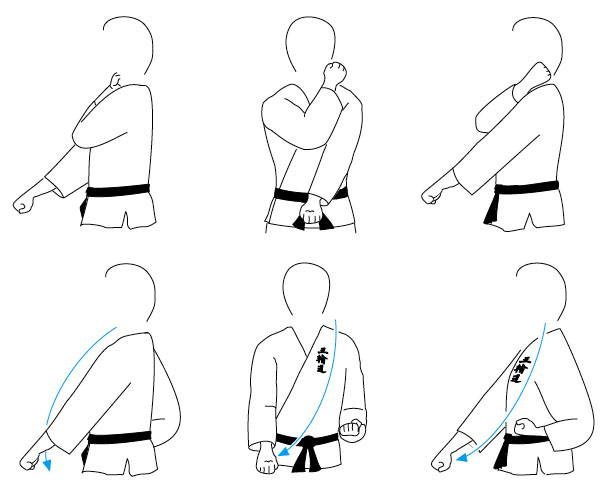
\includegraphics[width=0.5\textwidth]{images/gedanBarai}
	\label{fig:gedanBarai}
\end{figure}

%%%%%%%%%%%%%%%%%%%%%%%%%%%%%%%%%%%%%%%%%%%%%%%%%%%%%%%%%%%%%%%%%%%%%%%%%%%%%%%
\subsection{Setting}
Briefly explain what is supposed to happen want how the robot and human play a part in this.

%%%%%%%%%%%%%%%%%%%%%%%%%%%%%%%%%%%%%%%%%%%%%%%%%%%%%%%%%%%%%%%%%%%%%%%%%%%%%%%
% Hardware and Software
%%%%%%%%%%%%%%%%%%%%%%%%%%%%%%%%%%%%%%%%%%%%%%%%%%%%%%%%%%%%%%%%%%%%%%%%%%%%%%%
\section{Hardware and Software}

%%%%%%%%%%%%%%%%%%%%%%%%%%%%%%%%%%%%%%%%%%%%%%%%%%%%%%%%%%%%%%%%%%%%%%%%%%%%%%%
\subsection{Hardware}
In order to build this system the following components were used:
\begin{itemize}
  \item Laptop
  \item Nao robot
  \item Microsoft Kinect
\end{itemize}

The Microsoft Kinect is connected to the laptop using an USB cable and is used to capture the body model of the user. 

The Nao robot is controlled with a wireless connection using the wireless router. 

%%%%%%%%%%%%%%%%%%%%%%%%%%%%%%%%%%%%%%%%%%%%%%%%%%%%%%%%%%%%%%%%%%%%%%%%%%%%%%%
\subsection{Software}
In order to program this system the following software has been used:
\begin{itemize}
  \item Microsoft visual studio 2012
  \item Microsoft Kinect SDK
  \item Choregraph
\end{itemize}


%%%%%%%%%%%%%%%%%%%%%%%%%%%%%%%%%%%%%%%%%%%%%%%%%%%%%%%%%%%%%%%%%%%%%%%%%%%%%%%
% System
%%%%%%%%%%%%%%%%%%%%%%%%%%%%%%%%%%%%%%%%%%%%%%%%%%%%%%%%%%%%%%%%%%%%%%%%%%%%%%%
\section{System}
Discuss the system from an AI point of view.

%%%%%%%%%%%%%%%%%%%%%%%%%%%%%%%%%%%%%%%%%%%%%%%%%%%%%%%%%%%%%%%%%%%%%%%%%%%%%%%
\subsection{Perception}
A way to detect the user and the body model. Do not mention the Kinect.

%%%%%%%%%%%%%%%%%%%%%%%%%%%%%%%%%%%%%%%%%%%%%%%%%%%%%%%%%%%%%%%%%%%%%%%%%%%%%%%
\subsection{Communication}
Gestures + speech...

%%%%%%%%%%%%%%%%%%%%%%%%%%%%%%%%%%%%%%%%%%%%%%%%%%%%%%%%%%%%%%%%%%%%%%%%%%%%%%%
\subsection{World Model}



%%%%%%%%%%%%%%%%%%%%%%%%%%%%%%%%%%%%%%%%%%%%%%%%%%%%%%%%%%%%%%%%%%%%%%%%%%%%%%%
% Individual Components
%%%%%%%%%%%%%%%%%%%%%%%%%%%%%%%%%%%%%%%%%%%%%%%%%%%%%%%%%%%%%%%%%%%%%%%%%%%%%%%
\section{Individual Components}

\subsection{Perception}
Skeleton tracking + dynamic time warping

%%%%%%%%%%%%%%%%%%%%%%%%%%%%%%%%%%%%%%%%%%%%%%%%%%%%%%%%%%%%%%%%%%%%%%%%%%%%%%%
\subsection{Communication}

\subsubsection{Communication from robot to person}
In the communication from the robot to the person having the lesson both speech and gestures are used. 
Gestures are used during speaking to prevent the robot from looking way to static. 
During initial experiments it was noticed that people pay more attention to the robot when it is constantly actively moving. 

In the gestures used during speaker both beat gestures(gestures without semantic content) as well as metaphoric gestures (gestures indication thinking as well as gestures indication) are used. 

The metaphoric gestures that are used are:
\begin{itemize}
  \item Thinking
  \item Flexing of the muscles
  \item Bowing
\end{itemize}

The bowing gesture is used at the start of the program as bowing is a normal way to start any karate lesson. 
The thinking gesture is used after the user performed all motions, people reported that it fooled them thinking that the computer was computing the score during the gesture. 
The flexing of the muscles is used to show people how strong you are able to get by practicing a lot and is meant as motivation. 

Another way the robot communicates with the user is by making a short sound and lighting up its LEDs in its ears. 
When using the standard speech recognition in the robot this is standardly used to communicate to the user that it should now speak. 
As we used the Microsoft Kinect for speech recognition this sound was not needed anymore. 
During initial experiment we saw that people familiar with the robot would hesitate to speak as they thought the robot was not listening. 
By adding the blieb and lighting up its LEDs in its ears this problem was solved. 

During speeking the robot asks the user a lot of times to move his body the same way as the robot. 
This is done as initial experiments showed that users are hesitating to move along. 

The testing of all dialog is already done in an early phase of our project. 
During this phase a simple wizard of oz experiment was conducted in which the Kinect was not yet used. 
In order to fool people the Kinect was placed and connected to the computer to led the green indicater LED burn and the evaluation of a gesture was done at random. 
People did not notice and did indeed put extra effort in the performance of the gestures that the robot indicated needed improvement. 


\subsubsection{Communication from person to robot}
For speech a word-spotting algorithm is used.
This word-spotting algorithm uses a many-to-one mapping which maps several possible word onto one word that is returned to the system. 
This way the user can use several possible words to confirm a question of the robot. 
The mappings consist of: 
\begin{table}
  \begin{tabular}{|l|l|} \hline
    Keyword & Possible words           \\
    \hline 
    YES     & yes, sure, ETC.          \\
    NO      & no, nope, ETC.           \\
    LEFT    & left, left hand, ETC.    \\
    RIGHT   & right, right hand, ETC.  \\
    \hline
  \end{tabular}
\end{table}

During the program Naomi will ask the user for input several times. 
Some of the questions are used to keep the user active during the program and are just meant to give the user extra interaction with the robot. 
An example of this question is: ``Have you practiced Robot Karate before?'' after which the robot either will say that it will be an easy lesson or asks the user to give extra attention to the gestures. 

Other questions are used by the robot to give specific feedback.
An example of this question is asked during the performance of the defensive block: ``Are you having more trouble with your left or with your right arm'', after based on the input of the user the robot will explain only one arm of the defensive block. 



%%%%%%%%%%%%%%%%%%%%%%%%%%%%%%%%%%%%%%%%%%%%%%%%%%%%%%%%%%%%%%%%%%%%%%%%%%%%%%%
\subsection{World Model}

%%%%%%%%%%%%%%%%%%%%%%%%%%%%%%%%%%%%%%%%%%%%%%%%%%%%%%%%%%%%%%%%%%%%%%%%%%%%%%%
\subsection{Graphical User Interface}



%%%%%%%%%%%%%%%%%%%%%%%%%%%%%%%%%%%%%%%%%%%%%%%%%%%%%%%%%%%%%%%%%%%%%%%%%%%%%%%
% Interaction
%%%%%%%%%%%%%%%%%%%%%%%%%%%%%%%%%%%%%%%%%%%%%%%%%%%%%%%%%%%%%%%%%%%%%%%%%%%%%%%
\section{Interaction Patterns}


\begin{figure}[h!]
	\caption{State diagram showing in what order the behaviours of the robot are performed}
	\centering
	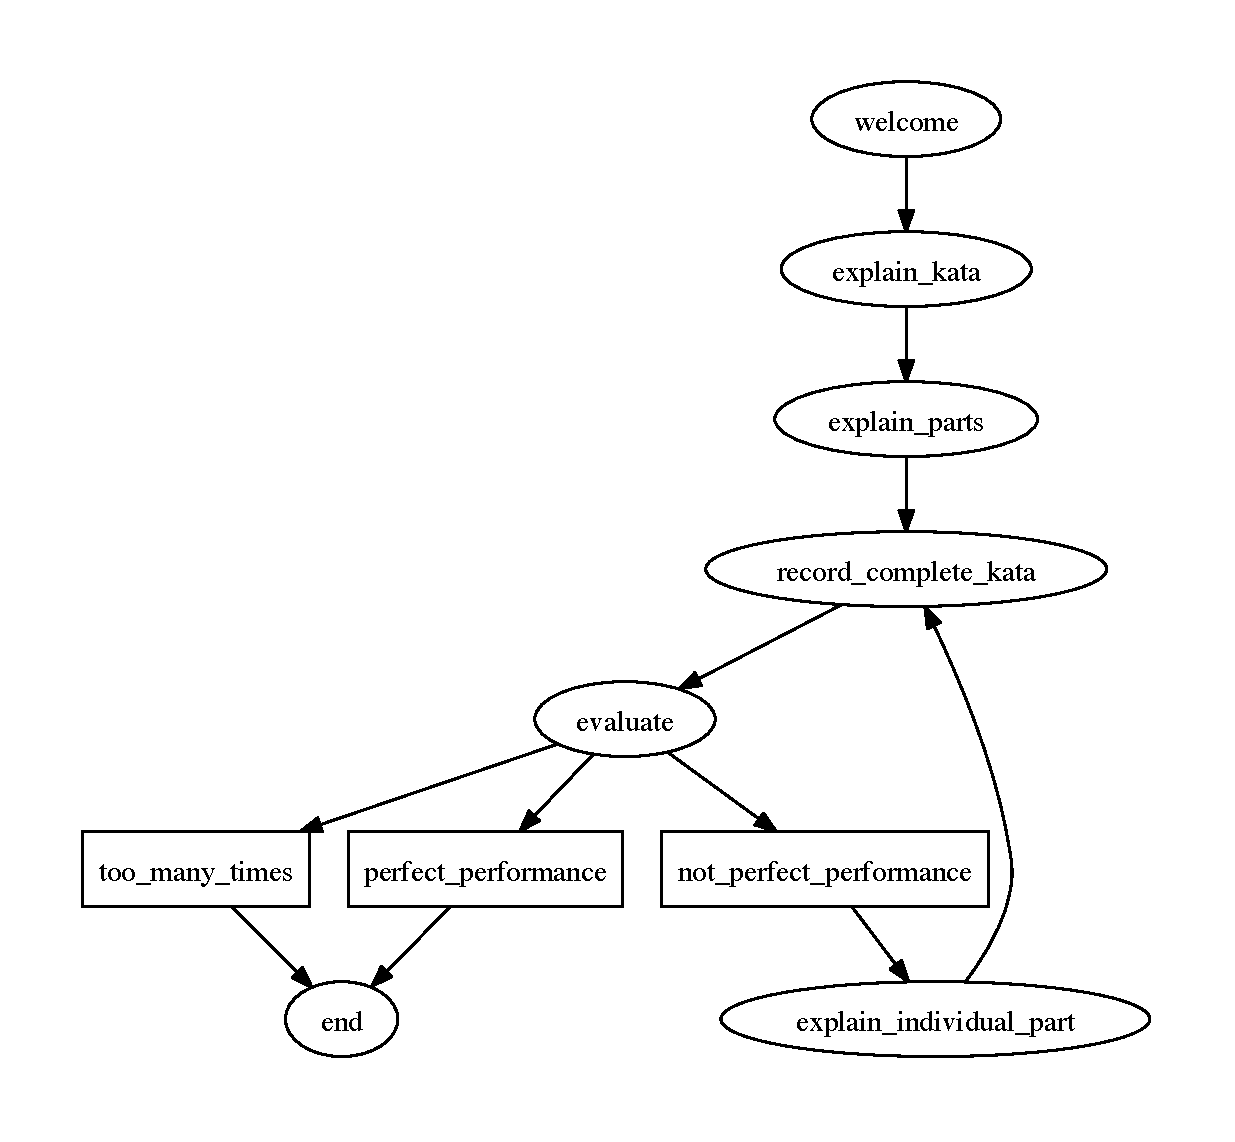
\includegraphics[width=0.5\textwidth]{images/stateDiagram}
	\label{fig:overviewTotalSystem}
\end{figure}

%%%%%%%%%%%%%%%%%%%%%%%%%%%%%%%%%%%%%%%%%%%%%%%%%%%%%%%%%%%%%%%%%%%%%%%%%%%%%%%
% Conclusion
%%%%%%%%%%%%%%%%%%%%%%%%%%%%%%%%%%%%%%%%%%%%%%%%%%%%%%%%%%%%%%%%%%%%%%%%%%%%%%%
\section{Conclusion}



%%%%%%%%%%%%%%%%%%%%%%%%%%%%%%%%%%%%%%%%%%%%%%%%%%%%%%%%%%%%%%%%%%%%%%%%%%%%%%%
% BIBLIOGRAPHY
%%%%%%%%%%%%%%%%%%%%%%%%%%%%%%%%%%%%%%%%%%%%%%%%%%%%%%%%%%%%%%%%%%%%%%%%%%%%%%%
\printbibliography

\end{document}
